\documentclass[border=12pt]{standalone}
% shared preamble for all schematics/diagrams
\usepackage[siunitx, RPvoltages, european resistors]{circuitikz}
\usepackage{tikz}
\usetikzlibrary{arrows.meta,positioning,calc,shapes.geometric,fit,backgrounds,decorations.pathreplacing}
\usepackage[scaled=0.92]{helvet}
\renewcommand{\familydefault}{\sfdefault}
\usepackage{xcolor}
\usepackage{amsmath}
\usepackage{ifthen}
\definecolor{ink}{HTML}{1F2328}
\definecolor{muted}{HTML}{6B6A66}
\definecolor{c1}{HTML}{2A78D6}
\definecolor{c2}{HTML}{EB6834}
\definecolor{c3}{HTML}{1BAF7A}
\definecolor{c4}{HTML}{6250D6}
\definecolor{fill1}{HTML}{EAF2FC}
\definecolor{fill2}{HTML}{FDEEE7}
\definecolor{fill3}{HTML}{E6F6EF}
\definecolor{fill4}{HTML}{EFEDFB}
\definecolor{hv}{HTML}{C62828}
\ctikzset{bipoles/thickness=1.2, monopoles/ground/thickness=1.2}
\tikzset{every picture/.style={line width=0.7pt, color=ink}}

\begin{document}
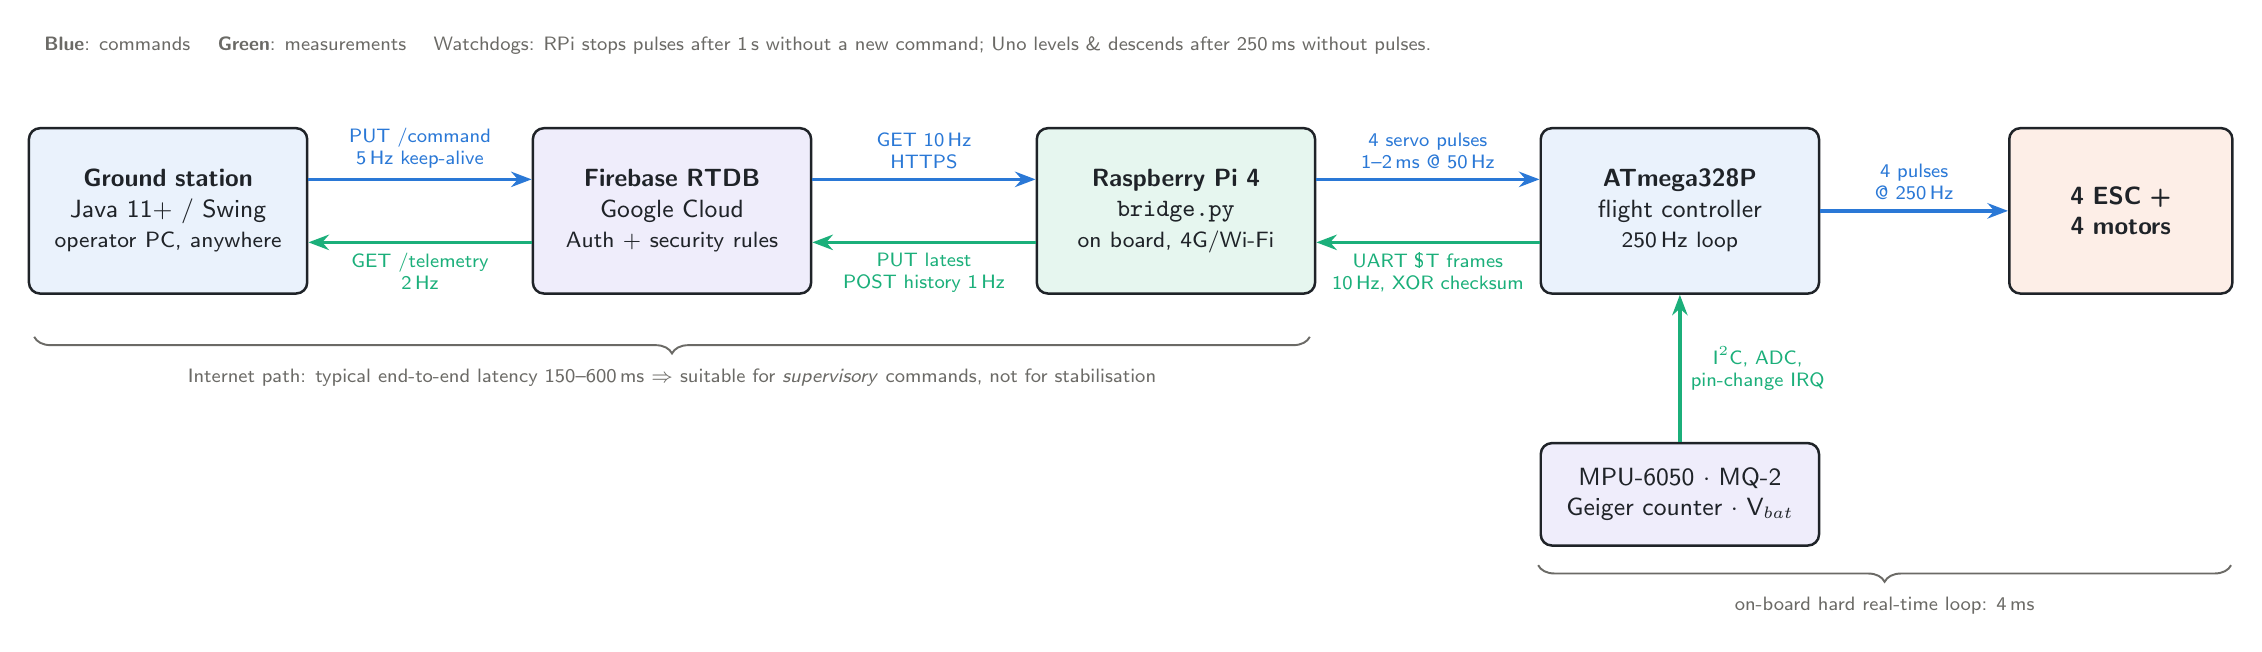
\begin{tikzpicture}[
  box/.style={draw, rounded corners=4pt, line width=0.9pt, fill=#1, align=center, minimum height=2.1cm, text width=3.3cm, font=\small},
  cmd/.style={line width=1.2pt, c1, -{Stealth[length=2.6mm]}},
  tel/.style={line width=1.2pt, c3, -{Stealth[length=2.6mm]}},
  note/.style={font=\scriptsize, align=center}]
\node[box=fill1] (gs) at (0,0) {\textbf{Ground station}\\Java 11+ / Swing\\\footnotesize operator PC, anywhere};
\node[box=fill4] (fb) at (6.4,0) {\textbf{Firebase RTDB}\\Google Cloud\\\footnotesize Auth + security rules};
\node[box=fill3] (rpi) at (12.8,0) {\textbf{Raspberry Pi 4}\\\texttt{bridge.py}\\\footnotesize on board, 4G/Wi-Fi};
\node[box=fill1] (fc) at (19.2,0) {\textbf{ATmega328P}\\flight controller\\\footnotesize 250\,Hz loop};
\node[box=fill2, text width=2.6cm] (esc) at (24.8,0) {\textbf{4 ESC +}\\\textbf{4 motors}};
\node[box=fill4, text width=3.3cm, minimum height=1.3cm] (sen) at (19.2,-3.6) {MPU-6050 $\cdot$ MQ-2\\Geiger counter $\cdot$ V$_{bat}$};

\draw[cmd] ([yshift=4mm]gs.east) -- ([yshift=4mm]fb.west) node[midway, above, note, c1] {PUT /command\\5\,Hz keep-alive};
\draw[cmd] ([yshift=4mm]fb.west -| fb.east) -- ([yshift=4mm]rpi.west) node[midway, above, note, c1] {GET 10\,Hz\\HTTPS};
\draw[cmd] ([yshift=4mm]rpi.east) -- ([yshift=4mm]fc.west) node[midway, above, note, c1] {4 servo pulses\\1--2\,ms @ 50\,Hz};
\draw[cmd] (fc.east) -- (esc.west) node[midway, above, note, c1] {4 pulses\\@ 250\,Hz};
\draw[tel] ([yshift=-4mm]fb.west) -- ([yshift=-4mm]gs.east) node[midway, below, note, c3] {GET /telemetry\\2\,Hz};
\draw[tel] ([yshift=-4mm]rpi.west) -- ([yshift=-4mm]fb.east) node[midway, below, note, c3] {PUT latest\\POST history 1\,Hz};
\draw[tel] ([yshift=-4mm]fc.west) -- ([yshift=-4mm]rpi.east) node[midway, below, note, c3] {UART \$T frames\\10\,Hz, XOR checksum};
\draw[tel] (sen) -- (fc) node[midway, right, note, c3] {I$^2$C, ADC,\\pin-change IRQ};

\draw[decorate, decoration={brace, amplitude=6pt, mirror}, muted] (-1.7,-1.6) -- (14.5,-1.6) node[midway, below=8pt, note, muted] {Internet path: typical end-to-end latency 150--600\,ms $\Rightarrow$ suitable for \emph{supervisory} commands, not for stabilisation};
\draw[decorate, decoration={brace, amplitude=6pt, mirror}, muted] (17.4,-4.5) -- (26.2,-4.5) node[midway, below=8pt, note, muted] {on-board hard real-time loop: 4\,ms};
\node[note, muted, anchor=west] at (-1.7,2.1) {\textbf{Blue}: commands \quad \textbf{Green}: measurements \quad Watchdogs: RPi stops pulses after 1\,s without a new command; Uno levels \& descends after 250\,ms without pulses.};
\end{tikzpicture}
\end{document}
